\documentclass[oneside]{tongjithesis} % 双面模式请将 oneside 改为 twoside
\usepackage{tongjithesis}
\usepackage{ulem}
\usepackage{makecell}
\begin{document}

\school{电子信息与工程学院}
\major{数据科学与大数据技术}
\student{}{范潇(2254298)}
\thesistitle{在 UNIX V6++中添加新的系统调用}{}
\thesistitleeng{Thesis Template}{with Various Scenes}
% \thesisadvisor{某某某}
\thesisdate{2024}{11}{13}

\MakeCover

\cleardoublepage

\pagestyle{firststyle}
% \MakeAbstract{
    摘要通常是一篇文章、论文、报告或其他文本的简短概括。它的目的是帮助读者了解文本的主要内容和结论,以便决定是否需要继续阅读原文。摘要通常包含文本的主题、目的、方法、结果和结论等方面的信息,并尽可能简洁明了地呈现。好的摘要应该能够概括文本的重点,同时避免使用不必要的细节和专业术语,以便广大读者能够轻松理解。

    此外,摘要通常也是学术界和研究人员评估一篇文献的重要依据之一。在文献检索和筛选过程中,人们通常会根据摘要来决定是否进一步查看完整的文献。因此,撰写一个清晰、准确、简洁的摘要对于文献的传播和影响力至关重要。在撰写摘要时,作者应该遵循文献的格式要求和撰写规范,同时结合文本的内容和目的,将摘要撰写得准确、简洁、易懂,以提高文献的传播和影响力。

    关键词1,关键词2,关键词3通常是与文章内容相关的几个词语,用于帮助读者更好地了解文章主题和内容。关键词的选择应该与文章的主题和研究领域密切相关,通常应该选择具有代表性、权威性、独特性和可搜索性的词语。
}{关键词1,关键词2,关键词3}

\MakeAbstractEng{
    An abstract is usually a short summary of an article, essay, report, or other text. Its purpose is to help the reader understand the main content and conclusions of the text so that he or she can decide whether he or she needs to continue reading the original text. The abstract usually contains information about the topic, purpose, methods, results, and conclusions of the text and is presented as concisely and clearly as possible. A good abstract should be able to summarize the main points of the text while avoiding unnecessary details and jargon so that it can be easily understood by a wide audience.

    In addition, abstracts are often one of the most important bases on which academics and researchers evaluate a piece of literature. During the literature search and selection process, people often base their decision to look further into the complete literature on the abstract. Therefore, writing a clear, accurate, and concise abstract is crucial to the dissemination and impact of the literature. When writing an abstract, authors should follow the formatting requirements and writing specifications of the literature, as well as combine the content and purpose of the text to write an accurate, concise, and easy-to-understand abstract in order to improve the dissemination and impact of the literature.

    Keyword 1, Keyword 2, and Keyword 3 are usually a few words related to the content of the article and are used to help readers better understand the topic and content of the article. The choice of keywords should be closely related to the topic and research area of the article, and words that are representative, authoritative, unique, and searchable should usually be chosen.
}{Keyword 1, Keyword 2, Keyword 3}


\clearpage
\tableofcontents   %放置目录
\cleardoublepage

\pagestyle{mainstyle}
\section{需求分析}\label{sec:demand}
\subsection{问题背景}
\subsubsection{共享单车的概念}
共享单车作为共享经济的新形态,
是指企业与政府进行合作,在居民区、商业区、地铁站、公交车
站、校园等公共场所提供自行车骑行的共享服务。它是借助互
联网技术推出的一种分时租赁业务。在整个运营过程中由智能
技术提供支持,企业负责整个运营过程中的管理\cite{article1}。
\subsubsection{共享单车企业面对的挑战}
消费者在选择共享单车品牌时,除了定价、押金等经济因素,还会着重考量以下体验因素:

\begin{itemize}
    \item 单车性能:例如单车重量,可调节性等;
    \item 维护质量:是否有大量未及时回收的损坏单车;
    \item 单车分布:单车的时空分布是否符合使用需求的时空分布。
\end{itemize}

同时,由于共享单车市场的快速发展,交通运输部等10部门也对共享单车(互联网租凭自行车)行业发布指导意见,要求“引导有序投放车辆”、“加强互联网租凭自行车标准化建设”、“加强停放管理和监督执法”,“引导用户安全文明用车”等。

为此,想要提高市场竞争力,占据主导地位,共享单车企业首先需要达成以下目标:

\begin{itemize}
    \item 及时更新迭代投入使用的单车型号;
    \item 追踪投入使用的单车的情况,如已使用时长;
    \item 记录并处理用户的反馈,例如单车损坏情况、用车需求;
    \item 及时回收损坏单车;
    \item 实时调度闲置单车至需求密集区域;
    \item 及时对违规停车用户进行处罚。
\end{itemize}

上述这些目标都可以纳入城市共享单车管理与调度的范畴之中。
\subsection{目标场景}
本次设计的数据库用于共享单车企业的共享单车管理与调度系统。因此,该数据库中存储的数据均围绕“共享单车”这一主体,
并不涉及用户的余额、购买的月卡套餐等信息。

下面列出的是本次设计的数据库的几个可能的使用场景:
\begin{itemize}
    \item 在共享单车手机应用中,需要使用该数据库中存储的数据来实时显示用户附近的可使用车辆信息;
    \item 共享单车运维团队定时根据数据库中存储的信息来回收并淘汰使用时间过长或型号过旧的单车;
    \item 共享单车运维团队定时从数据库中读取近期的用户反馈,并回收涉及的单车;
    \item 共享单车运维团队根据数据库中存储的行车记录,分析单车使用需求的时空分布,指定调度方案;
    % \item 共享单车企业根据数据库中存储的行车记录来动态调整推荐停车点的数量和位置;
    \item 分析团队利用数据库中存储的行车轨迹数据对用户使用习惯进行分析;
    \item 分析团队利用聚类等方式对数据库中存储的单车位置数据进行分析;
    \item 分析团队对数据库中存储的历史数据进行可视化。
\end{itemize}
\subsection{数据需求}
针对上述应用场景,本数据库存储和下列对象相关的数据:
\begin{itemize}
    \item 单车
    \item 单车轨迹
    \item 单车回收信息
    \item 单车调度信息
    \item 单车投放信息
    \item 用户
    \item 用户反馈
    % \item 停车点
    \item 仓库
\end{itemize}
% 具体属性已经各实体之间的关系将在后续的概念设计与逻辑设计中详细阐明。
\subsection{功能需求}
根据上述的应用场景,可知该数据库中需要进行的操作具有以下特点:
\begin{itemize}
    \item 经常需要根据时间属性进行范围选择,并且以附近的时间段为主;
    \item 需要针对空间数据,即坐标,进行范围查询,即获取一定范围内的数据;
    \item 更新单车回收、投放、调度信息时,需要同步更新单车坐标,仓库存储情况等数据;
    \item 特定数据更新频率较高,例如单车的当前坐标、状态信息;
    \item 有时需要读出大量数据,例如进行数据分析和可视化时;
    \item 较少进行删除操作。
\end{itemize}

在进行后续的设计时,将针对上述特点对数据库进行优化。
\clearpage
\section{概念设计}\label{sec:concept}
\subsection{E-R图}
根据上述的需求分析,在本次设计的数据库中,包含以下实体集:
\begin{itemize}
  \item \textit{bike}:拥有属性(\textit{\underline{bike\_ID},production\_date,coordinate,valid});
  \item \textit{collection}:拥有属性(\textit{\underline{collection\_ID},time});
  \item \textit{reallocation}:拥有属性(\textit{\dotuline{reallocation\_ID},start\_time,start\_coordinate,end\_time,end\_coordinate});
  \item \textit{release}:拥有属性(\textit{\underline{release\_ID},coordinate,time});
  \item \textit{trace}:拥有属性(\textit{\underline{trace\_ID},start\_time,start\_coordinate,end\_time,end\_coordinate});
  \item \textit{type}:拥有属性(\textit{\underline{type\_ID},name,release\_date});
  \item \textit{user}:拥有属性(\textit{\underline{user\_ID}});
  \item \textit{warehouse}:拥有属性(\textit{\underline{warehouse\_ID},capacity,load,coordinate}),
\end{itemize}
并且包含以下关系集:
\begin{itemize}
  \item \textit{bike\_collection}:将单车回收工单、单车和仓库关联在一起;
  \item \textit{bike\_reallocation}:将单车调度工单和单车关联在一起;
  \item \textit{bike\_release}:将单车投放工单、单车和仓库关联在一起;
  \item \textit{bike\_type}:将单车和单车型号关联在一起;
  \item \textit{stored\_in}:将单车和仓库关联在一起;
  \item \textit{usage}:将单车、单车轨迹和用户关联在一起;
  \item \textit{user\_feedback}:将单车和用户关联在一起,
\end{itemize}

图\ref{fig:E-R diagram}是由以上实体集和关系集组合形成的E-R图。

下面将对各个实体集和关系集展开介绍。
\begin{figure}[htbp]
  \centering
  \includegraphics{figures/E-R_diagram.pdf}
  \caption{E-R图}
  \label{fig:E-R diagram}
\end{figure}
\subsection{实体集设计}
\paragraph{\textit{bike}}
该实体集的拓展是在现实中公司所拥有的单车。

该实体集有以下属性:
\begin{itemize}
  \item \textit{\underline{bike\_ID}}:我们认为在同一家共享单车公司中,单车的序列号应当是唯一的,所以将其作为该实体集的主码;
  \item \textit{production\_date}:单车的生产日期;
  \item \textit{coordinate}:该属性用于追踪单车的当前坐标;
  \item \textit{valid}:该属性标记单车状态是否合法,当单车被发现遭到人为破坏、故意藏匿等情况,从而导致GPS失效、无法进行调度等情况时,将该属性值置为\textit{False}。
\end{itemize}

这里的\textit{production\_date,coordinate}实际上都是复合属性,例如\textit{coordinate}由经度和纬度组成,但是在该数据库的实际应用场景中,通常将它们
作为整体来使用,所以在概念设计中将它们视为整体。

\paragraph{\textit{collection}}
该实体集的拓展是在现实中公司的运转过程中所产生单车回收工单。这里针对以下两种工作流程进行设计:
\begin{itemize}
\item 系统会向调度员派发单车回收工单,调度员根据该工单将指定的单车回收至指定的仓库中;
\item 调度员自行收集单车,将其回收至特定仓库,并形成相应工单。
\end{itemize}

该实体集有以下属性:
\begin{itemize}
  \item \textit{\underline{collection\_ID}}:我们认为在同一家共享单车公司中,单车回收工单的序列号应当是唯一的,所以将其作为该实体集的主码;
  \item \textit{time}:完成该工单时的时间戳;
\end{itemize}

所收集的单车以及回收至的仓库这两个信息体现在关系集\textit{bike\_collection}中。
\paragraph{\textit{release}}
该实体集的拓展是在现实中公司的运转过程中所产生单车投放工单。这里针对以下工作流程进行设计:
\begin{itemize}
\item 调度员根据工单将一批指定的单车从仓库中运送至指定坐标。
\end{itemize}

该实体集有以下属性:
\begin{itemize}
  \item \textit{\underline{release\_ID}}:我们认为在同一家共享单车公司中,单车投放工单的序列号应当是唯一的,所以将其作为该实体集的主码;
  \item \textit{coordinate}:投放地点坐标;
  \item \textit{time}:完成该工单时的时间戳;
\end{itemize}

所投放的单车以及回收至的仓库这两个信息体现在关系集\textit{bike\_collection}中。
\paragraph{\textit{reallocation}}
该实体集的拓展是在现实中所产生的调度行为。

和\textit{collection,release}不同,该实体集的数据粒度更细,一个元组不再代表对于一批单车的操作,而是对单个单车的操作。这是因为调度
对精细化程度的要求通常更高。
我们认为同一单车调度工单可以涉及到多个单车,但是各个单车的最终投放地点和时间都可能不同。因此我将该实体集涉及为弱实体集,它的识别集是\textit{bike},识别关系集是\textit{bike\_reallocation}。

该实体集有以下属性:
\begin{itemize}
  \item \textit{\dotuline{reallocation\_ID}}:单车调度工单的序列号,作为该弱实体集的识别器;
  \item \textit{start\_time}:该调度操作的开始时间;
  \item \textit{start\_coordinate}:该调度操作的起始坐标;
  \item \textit{end\_time}:该调度操作的结束时间;
  \item \textit{end\_coordinate}:该调度操作的目的地坐标。
\end{itemize}
\paragraph{\textit{trace}}
该实体集的拓展是在现实中用户使用单车时所产生的单车轨迹。

该实体集有以下属性:
\begin{itemize}
  \item \textit{\underline{trace\_ID}}:我们认为在同一家共享单车公司中,单车轨迹的序列号应当是唯一的,所以将其作为该实体集的主码;
  \item \textit{start\_time}:轨迹起始时间;
  \item \textit{start\_coordinate}:轨迹起始坐标;
  \item \textit{end\_time}:轨迹结束时间;
  \item \textit{end\_coordinate}:轨迹结束坐标。
\end{itemize}
\paragraph{\textit{type}}
该实体集的拓展是在现实中企业所研发的共享单车型号。

该实体集有以下属性:
\begin{itemize}
  \item \textit{\underline{type\_ID}}:我们认为在同一家共享单车公司中,单车的型号代码应当是唯一的,所以将其作为该实体集的主码;
  \item \textit{name}:型号名称。这里我们假设不同型号可能有相同的名称,但是它们的代码是不同的;
  \item \textit{release\_time}:发布日期。
\end{itemize}
\paragraph{\textit{user}}
该实体集的拓展是在现实中企业所拥有的用户。

该实体集有以下属性:
\begin{itemize}
  \item \textit{\underline{user\_ID}}:我们认为在同一家共享单车公司中,用户ID应当是唯一的,所以将其作为该实体集的主码;
\end{itemize}

因为本数据库用于共享单车的管理与调度,所以无需将“用户余额”等属性添加入该实体集中。
\paragraph{\textit{warehouse}}
该实体集的拓展是在现实中企业所拥有的共享单车仓库。

该实体集有以下属性:
\begin{itemize}
  \item \textit{\underline{warehouse\_ID}}:我们认为在同一家共享单车公司中,仓库ID应当是唯一的,所以将其作为该实体集的主码;
  \item \textit{capacity}:仓库的最大存储容量;
  \item \textit{load}:仓库当前存储量;
  \item \textit{coordinate}:仓库坐标。这里我们假设两个仓库可能坐标相同,例如当仓库分为两层,或相邻很近时。
\end{itemize}
\subsection{关系集设计}
在本节中,我将图表中的实体集的属性略去。
\paragraph{\textit{bike\_collection}}
如图\ref{fig:bikecollection}所示,关系集\textit{bike\_collection}将实体集\textit{bike,collection,warehouse}联系在一起。

该关系集表达的是“单车依据单车收集工单被收集至指定仓库”这一事件中“单车”、“单车收集工单”和“仓库”之间的关系。这里使用了3元关系集,而非用若干个2元关系集进行代替,
是为了使得这三者之间的关系更加明确,并且避免进一步提升E-R图的复杂度\cite{dbconcept}。

\begin{figure}[htbp]
  \centering
  \includegraphics{figures/bike_collection.pdf}
  \caption{\textit{bike\_collection}}
  \label{fig:bikecollection}
\end{figure}

图中指向实体集\textit{warehouse}的箭头是指给定一个单车和相关联的单车收集工单,最多只有一个仓库与它们相关联。
\paragraph{\textit{bike\_reallocation}}
如图\ref{fig:bikereallocation}所示,关系集\textit{bike\_reallocation}将实体集\textit{bike,reallocation}联系在一起。

该关系集表达的是“调度单车”这一事件中“单车”和“调度行为”之间的关系。这里的\textit{reallocation}是弱实体集,它的存在依附于实体集\textit{bike}。因此,
实体集\textit{reallocation}完全参与关系集\textit{bike\_reallocation}。

\begin{figure}[htbp]
  \centering
  \includegraphics{figures/bike_reallocation.pdf}
  \caption{\textit{bike\_reallocation}}
  \label{fig:bikereallocation}
\end{figure}
\paragraph{\textit{bike\_release}}
如图\ref{fig:bikerelease}所示,关系集\textit{bike\_release}将实体集\textit{bike,release,warehouse}联系在一起。

该关系集表达的是“单车依据单车投放工单从指定仓库被投放至指定地点”这一事件中“单车”、“单车投放工单”和“仓库”之间的关系。和\textit{bike\_collection}一样,这里使用了3元关系集。

\begin{figure}[htbp]
  \centering
  \includegraphics{figures/bike_release.pdf}
  \caption{\textit{bike\_release}}
  \label{fig:bikerelease}
\end{figure}

图中指向实体集\textit{warehouse}的箭头是指给定一个单车和相关联的单车投放工单,最多只有一个仓库与它们相关联。由于可能有单车存放在仓库中尚未投入使用,
所以实体集\textit{bike}只部分参与该关系集。
\paragraph{\textit{bike\_type}}
如图\ref{fig:biketype}所示,关系集\textit{bike\_type}将实体集\textit{bike,type}联系在一起。

该关系集表达的是“任一单车都具有特定的型号”这一事实中“单车”与“型号”之间的关系。

\begin{figure}[htbp]
  \centering
  \includegraphics{figures/bike_type.pdf}
  \caption{\textit{bike\_type}}
  \label{fig:biketype}
\end{figure}

由于一辆单车有且仅有一个型号,所以图中有指向实体集\textit{type}的箭头,并且实体集\textit{bike}完全参与该关系集。
\paragraph{\textit{stored\_in}}
如图\ref{fig:storedin}所示,关系集\textit{sotred\_in}将实体集\textit{bike,warehouse}联系在一起。

该关系集表达的是“单车存储在仓库中”这一状态中,“单车”与“仓库”之间的关系。

\begin{figure}[htbp]
  \centering
  \includegraphics{figures/stored_in.pdf}
  \caption{\textit{stored\_in}}
  \label{fig:storedin}
\end{figure}

由于一辆单车至多存放在一个仓库中,所以图中有指向实体集\textit{warehouse}的箭头。
\paragraph{\textit{usage}}
如图\ref{fig:usage}所示,关系集\textit{usage}将实体集\textit{bike,user,trace}联系在一起。

该关系集表达的是“用户使用单车”这一过程中,“单车”、“用户”与“行车轨迹”之间的关系。

\begin{figure}[htbp]
  \centering
  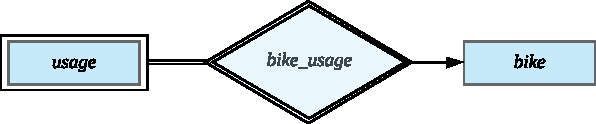
\includegraphics{figures/usage.pdf}
  \caption{\textit{usage}}
  \label{fig:usage}
\end{figure}

显然,实体集\textit{trace}应完全参与该关系集。
\paragraph{\textit{user\_feedback}}
如图\ref{fig:feedback}所示,关系集\textit{user\_feedback}将实体集\textit{bike,user}联系在一起。

该关系集表达的是“用户反馈单车故障”这一过程中,“单车”与“用户”之间的关系。

\begin{figure}[htbp]
  \centering
  \includegraphics{figures/user_feedback.pdf}
  \caption{\textit{user\_feedback}}
  \label{fig:feedback}
\end{figure}

用户反馈中的信息十分重要,这里我将反馈的时间\textit{time}和反馈的损坏器件\textit{component}作为该关系集的描述属性。因为
一次反馈可以反馈多处损坏,所以\textit{component}为多值属性。
\clearpage
% \input{sections/03_reference}
% \clearpage
\section{逻辑设计}\label{sec:logic}
\subsection{实体集模式}
\subsubsection{模式设计}
通过转换上述实体集,我们可以得到以下实体集模式:
\begin{table}[!hpt]
    \caption{实体集模式}
    \label{tab:entityschema}
    \centering
    \begin{tabular}{l} \toprule
         \textit{bike}(\textit{\underline{bike\_ID},production\_date,coordinate,valid})\\
         \textit{collection}(\textit{\underline{collection\_ID},time})\\
         \textit{reallocation}(\textit{\underline{reallocation\_ID},\underline{bike\_ID},start\_time,start\_coordinate,end\_time,end\_coordinate})\\
         \textit{release}(\textit{\underline{release\_ID},coordinate,time})\\
         \textit{trace}(\textit{\underline{trace\_ID},start\_time,start\_coordinate,end\_time,end\_coordinate})\\
         \textit{type}(\textit{\underline{type\_ID},name,release\_date})\\
         \textit{user}(\textit{\underline{user\_ID}})\\
         \textit{warehouse}(\textit{\underline{warehouse\_ID},capacity,load,coordinate}) \\ \bottomrule
    \end{tabular}
  \end{table}

  在转换过程中,我们认为坐标、日期以及时间都是不可分割的单元。在实际应用场景中,也常常将它们作为整体来进行使用。

  对于弱实体集\textit{reallocation},它的模式的主码由它自身的识别器\textit{reallocation\_ID}和
  识别集\textit{bike}的主码\textit{bike\_ID}组成;对于其余强实体集,它们的模式的主码和原来的主码保持一致。
\subsubsection{属性类型设计}
图\ref{tab:bike}-\ref{tab:warehouse}为各实体集模式中属性的类型。
\begin{figure}[!htp]
    \begin{minipage}{0.3\textwidth}
      \centering
      \caption{\textit{bike}模式属性类型}
      \label{tab:bike}
      \begin{tabular}{ll}\toprule
        属性&类型\\\midrule
       \textit{bike\_ID}&\textbf{char}(20)\\
       \textit{production\_date}&\textbf{date}\\
       \textit{coordinate}&\textbf{point}\\
       \textit{valid}&\textbf{int}\\
       \bottomrule
      \end{tabular}
    \end{minipage}\hfill
    \begin{minipage}{0.3\textwidth}
      \centering
      \caption{\textit{collection}模式属性类型}
      \label{tab:collection}
      \begin{tabular}{ll}\toprule
        属性&类型\\\midrule
       \textit{collection\_ID}&\textbf{char}(20)\\
       \textit{time}&\textbf{timestamp}\\
       \bottomrule
      \end{tabular}
    \end{minipage}\hfill
    \begin{minipage}{0.3\textwidth}
      \centering
      \caption{\textit{reallocation}模式属性类型}
      \label{tab:reallocation}
      \begin{tabular}{ll}\toprule
        属性&类型\\\midrule
       \textit{reallocation\_ID}&\textbf{char}(20)\\
       \textit{bike\_ID}&\textbf{char}(20)\\
       \textit{start\_time}&\textbf{timestamp}\\
       \textit{start\_coordinate}&\textbf{point}\\
       \textit{end\_time}&\textbf{timestamp}\\
       \textit{end\_coordinate}&\textbf{point}\\
       \bottomrule
      \end{tabular}
    \end{minipage}\hfill
  \end{figure}
\begin{figure}[!htp]
    \begin{minipage}{0.3\textwidth}
      \centering
      \caption{\textit{release}模式属性类型}
      \label{tab:release}
      \begin{tabular}{ll}\toprule
        属性&类型\\\midrule
       \textit{release\_ID}&\textbf{char}(20)\\
       \textit{coordinate}&\textbf{point}\\
       \textit{time}&\textbf{timestamp}\\
       \bottomrule
      \end{tabular}
    \end{minipage}\hfill
    \begin{minipage}{0.3\textwidth}
      \centering
      \caption{\textit{trace}模式属性类型}
      \label{tab:trace}
      \begin{tabular}{ll}\toprule
        属性&类型\\\midrule
       \textit{trace\_ID}&\textbf{char}(20)\\
       \textit{start\_time}&\textbf{timestamp}\\
       \textit{start\_coordinate}&\textbf{point}\\
       \textit{end\_time}&\textbf{timestamp}\\
       \textit{end\_coordinate}&\textbf{point}\\
       \bottomrule
      \end{tabular}
    \end{minipage}\hfill
    \begin{minipage}{0.3\textwidth}
      \centering
      \caption{\textit{type}模式属性类型}
      \label{tab:type}
      \begin{tabular}{ll}\toprule
        属性&类型\\\midrule
       \textit{type\_ID}&\textbf{char}(5)\\
       \textit{name}&\textbf{varchar}(50)\\
       \textit{release\_date}&\textbf{date}\\
       \bottomrule
      \end{tabular}
    \end{minipage}\hfill
  \end{figure}
\begin{figure}[!htp]
    \begin{minipage}{0.45\textwidth}
      \centering
      \caption{\textit{user}模式属性类型}
      \label{tab:user}
      \begin{tabular}{ll}\toprule
        属性&类型\\\midrule
       \textit{user\_ID}&\textbf{char}(20)\\
       \bottomrule
      \end{tabular}
    \end{minipage}\hfill
    \begin{minipage}{0.45\textwidth}
      \centering
      \caption{\textit{warehouse}模式属性类型}
      \label{tab:warehouse}
      \begin{tabular}{ll}\toprule
        属性&类型\\\midrule
       \textit{warehouse\_ID}&\textbf{char}(10)\\
       \textit{capacity}&\textbf{int}\\
       \textit{load}&\textbf{int}\\
       \textit{coordinate}&\textbf{point}\\
       \bottomrule
      \end{tabular}
    \end{minipage}\hfill
  \end{figure}

对于设计过程,有以下几点说明:
\begin{itemize}
    \item 使用MySQL等数据库所支持的\textbf{point}类型来表示坐标信息;
    \item 假设\textit{bike\_ID}等识别码是定长的,所以将它们的类型设为\textbf{char}。由于单车类型和仓库的数量较少,所以\textit{type\_ID,warehouse\_ID}分别的类型分别设为\textbf{char(5)},\textbf{char(10)}。
\end{itemize}
\subsection{关系集模式}
\subsubsection{模式设计}
通过转换上述关系集,我们可以得到以下关系集模式:
\begin{table}[!hpt]
    \caption{关系集模式}
    \label{tab:relationschema}
    \centering
    \begin{tabular}{l} \toprule
         \textit{bike\_collection}(\textit{\underline{bike\_ID},\underline{collection\_ID}})\\
         \textit{collection\_warehouse}(\textit{\underline{collection\_ID},warehouse\_ID})\\
        %  \textit{bike\_reallocation}(\textit{\underline{reallocation\_ID},\underline{bike\_ID}})\\
         \textit{bike\_release}(\textit{\underline{bike\_ID},\underline{release\_ID}})\\
         \textit{release\_warehouse}(\textit{\underline{release\_ID},warehouse\_ID})\\
         \textit{bike\_type}(\textit{\underline{bike\_ID},type\_ID})\\
         \textit{stored\_in}(\textit{\underline{bike\_ID},warehouse\_ID})\\
         \textit{usage}(\textit{\underline{trace\_ID},user\_ID,bike\_ID})\\
         \textit{user\_feedback}(\textit{\underline{user\_ID},\underline{bike\_ID},\underline{time}})\\
         \textit{feedback\_component}(\textit{\underline{user\_ID},\underline{bike\_ID},\underline{time},\underline{component}})\\
         \bottomrule
    \end{tabular}
  \end{table}

  在转换的过程中,联系弱实体集\textit{reallocation}和其识别集\textit{bike}的关系集\textit{bike\_reallocation}被略去,因为这是冗余的\cite{dbconcept2}。
  同时,我将三元关系集\textit{bike\_collection,bike\_release}分别拆分为了两个模式,这是为了保证模式满足第二范式,否则,属性\textit{warehouse}将会部分依赖于主码\textit{collection\_ID,bike\_ID}中的\textit{collection\_ID}和主码\textit{release\_ID,bike\_ID}中的\textit{release\_ID}。

  对于“多对一”和“一对多”的二元关系集,它的模式的主码为“多”那一侧的实体集模式的主码;对于“多对多”的二元关系集,它的主码是它关联起来的实体集模式的主码与它的描述属性的并集;对于“一对一”的二元关系集,
  它的主码可以是它关联起来的任一实体集的主码\cite{dbconcept3}。表\ref{tab:relationschema}中模式的主码便是按照上述标准进行选取的。

  对于三元关系集\textit{usage},我则是按照函数依赖来选择它们的模式的主码。

  对于关系集\textit{user\_feedback},它的描述属性之一\textit{component}是多值属性。为此,转换为模式时,额外创建一个模式\textit{feedback\_component},
  其属性由\textit{user\_feedback}的主码以及属性\textit{component}组成。
\subsubsection{属性类型设计}
关系集模式中属性的类型与实体集中的相应属性类型保持一致。图\ref{tab:bikecollection}-\ref{tab:feedbackcomponent}为各实体集模式中属性的类型。
\begin{figure}[!htp]
    \begin{minipage}{0.3\textwidth}
      \centering
      \caption{\textit{bike\_collection}模式属性类型}
      \label{tab:bikecollection}
      \begin{tabular}{ll}\toprule
        属性&类型\\\midrule
       \textit{collection\_ID}&\textbf{char}(20)\\
       \textit{bike\_ID}&\textbf{char}(20)\\
       \bottomrule
      \end{tabular}
    \end{minipage}\hfill
    \begin{minipage}{0.3\textwidth}
      \centering
      \caption{\textit{collection\_warehouse}模式属性类型}
      \label{tab:collectionwarehouse}
      \begin{tabular}{ll}\toprule
        属性&类型\\\midrule
       \textit{collection\_ID}&\textbf{char}(20)\\
       \textit{warehouse\_ID}&\textbf{char}(10)\\
       \bottomrule
      \end{tabular}
    \end{minipage}\hfill
    \begin{minipage}{0.3\textwidth}
      \centering
      \caption{\textit{bike\_release}模式属性类型}
      \label{tab:bikerelease}
      \begin{tabular}{ll}\toprule
        属性&类型\\\midrule
       \textit{bike\_ID}&\textbf{char}(20)\\
       \textit{release\_ID}&\textbf{char}(20)\\
       \bottomrule
      \end{tabular}
    \end{minipage}\hfill
\end{figure}

\begin{figure}[!htp]
    \begin{minipage}{0.3\textwidth}
      \centering
      \caption{\textit{release\_warehouse}模式属性类型}
      \label{tab:releasewarehouse}
      \begin{tabular}{ll}\toprule
        属性&类型\\\midrule
       \textit{release\_ID}&\textbf{char}(20)\\
       \textit{warehouse\_ID}&\textbf{char}(10)\\
       \bottomrule
      \end{tabular}
    \end{minipage}\hfill
    \begin{minipage}{0.3\textwidth}
      \centering
      \caption{\textit{bike\_type}模式属性类型}
      \label{tab:biketype}
      \begin{tabular}{ll}\toprule
        属性&类型\\\midrule
       \textit{type\_ID}&\textbf{char}(5)\\
       \textit{bike\_ID}&\textbf{char}(20)\\
       \bottomrule
      \end{tabular}
    \end{minipage}\hfill
    \begin{minipage}{0.3\textwidth}
      \centering
      \caption{\textit{stored\_in}模式属性类型}
      \label{tab:storedin}
      \begin{tabular}{ll}\toprule
        属性&类型\\\midrule
       \textit{warehouse\_ID}&\textbf{char}(10)\\
       \textit{bike\_ID}&\textbf{char}(20)\\
       \bottomrule
      \end{tabular}
    \end{minipage}\hfill
  \end{figure}

\begin{figure}[!htp]
    \begin{minipage}{0.3\textwidth}
      \centering
      \caption{\textit{usage}模式属性类型}
      \label{tab:usage}
      \begin{tabular}{ll}\toprule
        属性&类型\\\midrule
       \textit{trace\_ID}&\textbf{char}(20)\\
       \textit{user\_ID}&\textbf{char}(20)\\
       \textit{bike\_ID}&\textbf{char}(20)\\
       \bottomrule
      \end{tabular}
    \end{minipage}\hfill
    \begin{minipage}{0.3\textwidth}
      \centering
      \caption{\textit{user\_feedback}模式属性类型}
      \label{tab:userfeedback}
      \begin{tabular}{ll}\toprule
        属性&类型\\\midrule
       \textit{user\_ID}&\textbf{char}(20)\\
       \textit{bike\_ID}&\textbf{char}(20)\\
       \textit{time}&\textbf{timestamp}\\
       \bottomrule
      \end{tabular}
    \end{minipage}\hfill
    \begin{minipage}{0.3\textwidth}
      \centering
      \caption{\textit{feedback\_component}模式属性类型}
      \label{tab:feedbackcomponent}
      \begin{tabular}{ll}\toprule
        属性&类型\\\midrule
       \textit{user\_ID}&\textbf{char}(20)\\
       \textit{bike\_ID}&\textbf{char}(20)\\
       \textit{time}&\textbf{timestamp}\\
       \textit{component}&\textbf{varchar}(50)\\
       \bottomrule
      \end{tabular}
    \end{minipage}\hfill
  \end{figure}
\subsection{约束设计}
约束设计主要分为两部分:外码约束和其他约束。

\paragraph{外码约束}
外码约束主要有三个来源:
\begin{enumerate}
    \item 关系集转化为关系集模式时所产生的;
    \item 转化复杂类型时所产生的;
    \item 转化弱实体集时所产生的。
\end{enumerate}

在本数据库中,关系集\textit{user\_feedback}的多值描述属性\textit{component}要求我们在将该关系集转化为模式时,需额外生成模式\textit{feedback\_component},
同时,\textit{feedback\_component}中的属性\textit{user\_ID,bike\_ID,time}遵循外码约束,引用\textit{user\_feedback}的主码。

在本数据库中,弱实体集\textit{reallocation}转换为模式\textit{reallocation},该模式中的属性\textit{bike\_ID}需遵循外码约束,引用模式\textit{bike}的主码。

其余外码约束均来自于由关系集转化而来的关系集模式。这些模式需要引用它对应的关系集所联系起来的实体集的主码。%特别地,对于由三元关系集\textit{bike\_collection}转化成的
% 模式\textit{bike\_collection}和\textit{collection\_warehouse},以及由三元关系集\textit{bike\_release}转化成的
% 模式\textit{bike\_release}和\textit{release\_warehouse},我们要求\textit{bike\_collection}需要引用\textit{collection\_warehouse},\textit{bike\_release}需要引用\textit{release\_warehouse}。

\paragraph{其他约束}
本数据库中的其他约束包括主码约束(非空且唯一)、非空约束、唯一约束,check约束。

由于本数据库中除了用户反馈外的其他所有数据理论上都可以由相应的设备自动生成,如行车轨迹,又或者是必不可少的一部分,例如仓库的坐标,所以所有属性都遵循非空约束。

对于坐标、时间戳等数据,我们不作唯一约束要求。

在本数据库中,check约束主要用于以下两处:
\begin{enumerate}
    \item 因为对于\textit{bike}中的\textit{valid}属性,我们用\textbf{int}类型来代替布尔类型,所以需要用check约束来确保该属性的取值为0或1;
    \item 理论上需要用check约束来确保用户反馈中填写的\textit{component}值是合法的,即属于给定的集合之中。但是这也可以在应用层面实现,例如只允许用户通过勾选的方式来进行反馈。
\end{enumerate}

图\ref{tab:constraintbike}-\ref{tab:cfeedbackcomponent}为各模式中的属性所需遵循的约束。
  图\ref{tab:cfeedbackcomponent}中的\textit{valid\_component}为一个常量,含义是合法的单车部件。

\begin{figure}[!htp]
    \begin{minipage}{0.3\textwidth}
      \centering
      \caption{\textit{bike}模式属性约束}
      \label{tab:constraintbike}
      \begin{tabular}{ll}\toprule
        属性&约束\\\midrule
       \textit{bike\_ID}&\textbf{primary key}\\
       \textit{production\_date}&\textbf{not null}\\
       \textit{coordinate}&\textbf{not null}\\
       \textit{valid}&\textbf{check}(valid \textbf{in} (0,1))\\
       \bottomrule
      \end{tabular}
    \end{minipage}\hfill
    \begin{minipage}{0.3\textwidth}
      \centering
      \caption{\textit{collection}模式属性约束}
      \label{tab:constraintcollection}
      \begin{tabular}{ll}\toprule
        属性&约束\\\midrule
       \textit{collection\_ID}&\textbf{primary key}\\
       \textit{time}&\textbf{not null}\\
       \bottomrule
      \end{tabular}
    \end{minipage}\hfill
    \begin{minipage}{0.3\textwidth}
      \centering
      \caption{\textit{reallocation}模式属性约束}
      \label{tab:constraintreallocation}
      \begin{tabular}{ll}\toprule
        属性&约束\\\midrule
       \textit{reallocation\_ID}&\textbf{primary key}\\
       \textit{bike\_ID}&\makecell[l]{\textbf{primary key}\\\textbf{references} \textit{bike}}\\
       \textit{start\_time}&\textbf{not null}\\
       \textit{start\_coordinate}&\textbf{not null}\\
       \textit{end\_time}&\textbf{not null}\\
       \textit{end\_coordinate}&\textbf{not null}\\
       \bottomrule
      \end{tabular}
    \end{minipage}\hfill
  \end{figure}
\begin{figure}[!htp]
    \begin{minipage}{0.3\textwidth}
      \centering
      \caption{\textit{release}模式属性约束}
      \label{tab:constraintrelease}
      \begin{tabular}{ll}\toprule
        属性&约束\\\midrule
       \textit{release\_ID}&\textbf{primary key}\\
       \textit{coordinate}&\textbf{not null}\\
       \textit{time}&\textbf{not null}\\
       \bottomrule
      \end{tabular}
    \end{minipage}\hfill
    \begin{minipage}{0.3\textwidth}
      \centering
      \caption{\textit{trace}模式属性约束}
      \label{tab:constrainttrace}
      \begin{tabular}{ll}\toprule
        属性&约束\\\midrule
       \textit{trace\_ID}&\textbf{primary key}\\
       \textit{start\_time}&\textbf{not null}\\
       \textit{start\_coordinate}&\textbf{not null}\\
       \textit{end\_time}&\textbf{not null}\\
       \textit{end\_coordinate}&\textbf{not null}\\
       \bottomrule
      \end{tabular}
    \end{minipage}\hfill
    \begin{minipage}{0.3\textwidth}
      \centering
      \caption{\textit{type}模式属性约束}
      \label{tab:constrainttype}
      \begin{tabular}{ll}\toprule
        属性&约束\\\midrule
       \textit{type\_ID}&\textbf{primary key}\\
       \textit{name}&\textbf{not null}\\
       \textit{release\_date}&\textbf{not null}\\
       \bottomrule
      \end{tabular}
    \end{minipage}\hfill
  \end{figure}
\begin{figure}[!htp]
    \begin{minipage}{0.3\textwidth}
      \centering
      \caption{\textit{user}模式属性约束}
      \label{tab:constraintuser}
      \begin{tabular}{ll}\toprule
        属性&约束\\\midrule
       \textit{user\_ID}&\textbf{primary key}\\
       \bottomrule
      \end{tabular}
    \end{minipage}\hfill
    \begin{minipage}{0.3\textwidth}
      \centering
      \caption{\textit{warehouse}模式属性约束}
      \label{tab:constraintwarehouse}
      \begin{tabular}{ll}\toprule
        属性&约束\\\midrule
       \textit{warehouse\_ID}&\textbf{primary key}\\
       \textit{capacity}&\textbf{not null}\\
       \textit{load}&\textbf{not null}\\
       \textit{coordinate}&\textbf{not null}\\
       \bottomrule
      \end{tabular}
    \end{minipage}\hfill
    \begin{minipage}{0.3\textwidth}
      \centering
      \caption{\textit{bike\_collection}模式属性约束}
      \label{tab:cbikecollection}
      \begin{tabular}{ll}\toprule
        属性&约束\\\midrule
       \textit{collection\_ID}&\makecell[l]{\textbf{primary key}\\\textbf{references} \textit{collection}}\\
       \textit{bike\_ID}&\makecell[l]{\textbf{primary key}\\\textbf{references} \textit{bike}}\\
       \bottomrule
      \end{tabular}
    \end{minipage}\hfill
 \end{figure}
  \begin{figure}[!htp]
    \begin{minipage}{0.3\textwidth}
      \centering
      \caption{\textit{collection\_warehouse}模式属性约束}
      \label{tab:ccollectionwarehouse}
      \begin{tabular}{ll}\toprule
        属性&约束\\\midrule
       \textit{collection\_ID}&\makecell[l]{\textbf{primary key}\\\textbf{references} \textit{collection}}\\
       \textit{warehouse\_ID}&\makecell[l]{\textbf{not null}\\\textbf{references} \textit{warehouse}}\\
       \bottomrule
      \end{tabular}
    \end{minipage}\hfill
    \begin{minipage}{0.3\textwidth}
      \centering
      \caption{\textit{bike\_release}模式属性约束}
      \label{tab:cbikerelease}
      \begin{tabular}{ll}\toprule
        属性&约束\\\midrule
       \textit{release\_ID}&\makecell[l]{\textbf{primary key}\\\textbf{references} \textit{release}}\\
       \textit{bike\_ID}&\makecell[l]{\textbf{primary key}\\\textbf{references} \textit{bike}}\\
       \bottomrule
      \end{tabular}
    \end{minipage}\hfill
    \begin{minipage}{0.3\textwidth}
      \centering
      \caption{\textit{release\_warehouse}模式属性约束}
      \label{tab:creleasewarehouse}
      \begin{tabular}{ll}\toprule
        属性&约束\\\midrule
       \textit{release\_ID}&\makecell[l]{\textbf{primary key}\\\textbf{references} \textit{release}}\\
       \textit{warehouse\_ID}&\makecell[l]{\textbf{not null}\\\textbf{references} \textit{warehouse}}\\
       \bottomrule
      \end{tabular}
    \end{minipage}\hfill
  \end{figure}
\begin{figure}[!htp]
    \begin{minipage}{0.3\textwidth}
      \centering
      \caption{\textit{bike\_type}模式属性约束}
      \label{tab:cbiketype}
      \begin{tabular}{ll}\toprule
        属性&约束\\\midrule
       \textit{bike\_ID}&\makecell[l]{\textbf{primary key}\\\textbf{references} \textit{bike}}\\
       \textit{type\_ID}&\makecell[l]{\textbf{not null}\\\textbf{references} \textit{type}}\\
       \bottomrule
      \end{tabular}
    \end{minipage}\hfill
    \begin{minipage}{0.3\textwidth}
      \centering
      \caption{\textit{stored\_in}模式属性约束}
      \label{tab:cstoredin}
      \begin{tabular}{ll}\toprule
        属性&约束\\\midrule
       \textit{bike\_ID}&\makecell[l]{\textbf{primary key}\\\textbf{references} \textit{bike}}\\
       \textit{warehouse\_ID}&\makecell[l]{\textbf{not null}\\\textbf{references} \textit{warehouse}}\\
       \bottomrule
      \end{tabular}
    \end{minipage}\hfill
    \begin{minipage}{0.3\textwidth}
      \centering
      \caption{\textit{usage}模式属性约束}
      \label{tab:cusage}
      \begin{tabular}{ll}\toprule
        属性&约束\\\midrule
       \textit{trace\_ID}&\makecell[l]{\textbf{primary key}\\\textbf{references} \textit{trace}}\\
       \textit{user\_ID}&\makecell[l]{\textbf{not null}\\\textbf{references} \textit{user}}\\
       \textit{bike\_ID}&\makecell[l]{\textbf{not null}\\\textbf{references} \textit{bike}}\\
       \bottomrule
      \end{tabular}
    \end{minipage}\hfill
  \end{figure}
  \begin{figure}
    \begin{minipage}{0.3\textwidth}
      \centering
      \caption{\textit{user\_feedback}模式属性约束}
      \label{tab:cuserfeedback}
      \begin{tabular}{ll}\toprule
        属性&约束\\\midrule
       \textit{user\_ID}&\makecell[l]{\textbf{primary key}\\\textbf{references} \textit{user}}\\
       \textit{bike\_ID}&\makecell[l]{\textbf{primary key}\\\textbf{references} \textit{bike}}\\
       \textit{time}&\textbf{primary key}\\
       \bottomrule
      \end{tabular}
    \end{minipage}\hfill
    \begin{minipage}{0.6\textwidth}
    \centering
      \caption{\textit{feedback\_component}模式属性约束}
      \label{tab:cfeedbackcomponent}
      \begin{tabular}{ll}\toprule
        属性&约束\\\midrule
       \textit{user\_ID}&\makecell[l]{\textbf{primary key}\\\textbf{references} \textit{user}}\\
       \textit{bike\_ID}&\makecell[l]{\textbf{primary key}\\\textbf{references} \textit{bike}}\\
       \textit{time}&\textbf{primary key}\\
       \textit{component}&\makecell[l]{\textbf{primary key}\\(\textbf{check} \textit{component} \textbf{in} \textit{valid\_component})}\\
    %    \bottomrule
       (\textit{user\_ID,bike\_ID,time})&\makecell[l]{\textbf{references} \textit{user\_feedback}}\\
       \bottomrule
      \end{tabular}
    \end{minipage}\hfill
  \end{figure}
  \subsection{范式分析}
  \subsubsection{第一范式}
  在从E-R图转换至模式的过程中,我已经将复杂属性拆分开来,所以所有模式满足第一范式。
  \subsubsection{第二范式}
  各个模式的函数依赖集的正则覆盖如下:
  \begin{table}[!hpt]
    \caption{各模式中的函数依赖的正则覆盖}
    \label{tab:functiondependency}
    \centering
    \begin{tabular}{l} \toprule
        $FC_{bike}=\{bike\_ID\rightarrow production\_date,coordinate,valid\}$\\
        $FC_{collection}=\{collection\_ID\rightarrow time\}$\\
        $FC_{reallocation}=\{reallocation\_ID,bike\_ID\rightarrow start\_time,start\_coordinate,end\_time,end\_coordinate\}$\\
        $FC_{release}=\{release\_ID\rightarrow coordinate,time\}$\\
        $FC_{trace}=\{trace\_ID\rightarrow start\_time,start\_coordinate,end\_time,end\_coordinate\}$\\
        $FC_{type}=\{type\_ID\rightarrow name,release\_date\}$\\
        $FC_{user}=\varnothing$\\
        $FC_{warehouse}=\{warehouse\_ID\rightarrow capacity,load,coordinate\}$\\
        $FC_{bike\_collection}=\varnothing$\\
        $FC_{collection\_warehouse}=\{collection\_ID\rightarrow warehouse\_ID\}$\\
        $FC_{bike\_release}=\varnothing$\\
        $FC_{release\_warehouse}=\{release\_ID\rightarrow warehouse\_ID\}$\\
        $FC_{bike\_type}=\{bike\_ID\rightarrow type\_ID\}$\\
        $FC_{stored\_in}=\{bike\_ID\rightarrow warehouse\_ID\}$\\
        $FC_{usage}=\{trace\_ID\rightarrow user\_ID,bike\_ID\}$\\
        $FC_{user\_feedback}=\varnothing$\\
        $FC_{feedback\_component}=\varnothing$\\
         \bottomrule
    \end{tabular}
 \end{table}

    经过验证,各个模式中不存在部分函数依赖,即所有模式满足第二范式。
    \subsubsection{第三范式}
    经过验证,各个模式中不存在传递依赖的关系,即所有模式满足第三范式。
    \subsubsection{BC范式}
    经过验证,所有模式满足BC范式。
 
    
\clearpage
\section{物理设计}\label{sec:physics}
\subsection{索引类型选择}
对于本次设计的数据库而言,绝大部分数据具有时序性,并且是按照时间顺序进行插入的。同时,在实际应用中很少对这些具有时序性的数据进行更新和
删除的操作。因此,即使存储的数据量较大,当使用顺序存储时,溢出块的数量能够维持在可控范围内。并且在夜间时,该数据库的输入频率将会处于低位,
数据库可以利用这一时间对数据进行重新组织。并且,对于具有时序性的数据,在实际应用中常常使用范围查找。综上,对于具有时序性的数据,
本数据库中主要对其建立顺序索引。

另一方面,对于\textit{bike}等模式,在实际应用中常常需要以坐标为条件进行查询,因此对于这些模式,需要使用k-d树或k-d-B树等专门用于处理
位置信息的索引类型。对于$bike\_ID$等识别码,在实际应用中常常以等值查询为主,它们的索引以哈希索引为主。
\subsection{索引设计}
在创建索引时,主要遵循以下几点:
\begin{enumerate}
  \item 对主码建立索引,以提高检查主码约束的效率;
  \item 对被引用的属性建立索引,以提高检查外码约束的效率;
  \item 对实际应用中查询频率高或响应时间要求高的属性建立索引。
\end{enumerate}

本数据库中各个模式中的索引信息如图\ref{tab:indexbike}-\ref{tab:indexfeedbackcomponent}所示。

\begin{figure}[!htp]
    \begin{minipage}{0.3\textwidth}
      \centering
      \caption{\textit{bike}模式索引信息}
      \label{tab:indexbike}
      \begin{tabular}{ll}\toprule
        属性&索引信息\\\midrule
       \textit{bike\_ID}&hash index\\
       \textit{production\_date}&primary index\\
       \textit{coordinate}&k-d tree\\
       \textit{valid}&\makecell[c]{——}\\
       \bottomrule
      \end{tabular}
    \end{minipage}\hfill
    \begin{minipage}{0.3\textwidth}
      \centering
      \caption{\textit{collection}模式索引信息}
      \label{tab:indexollection}
      \begin{tabular}{ll}\toprule
        属性&索引信息\\\midrule
       \textit{collection\_ID}&hash index\\
       \textit{time}&primary index\\
       \bottomrule
      \end{tabular}
    \end{minipage}\hfill
    \begin{minipage}{0.3\textwidth}
      \centering
      \caption{\textit{reallocation}模式索引信息}
      \label{tab:indexreallocation}
      \begin{tabular}{ll}\toprule
        属性&索引信息\\\midrule
       \textit{reallocation\_ID}&hash index\\
       \textit{bike\_ID}&hash index\\
       \textit{start\_time}&primary index\\
       \textit{start\_coordinate}&k-d tree\\
       \textit{end\_time}&secondary index\\
       \textit{end\_coordinate}&k-d tree\\
       \bottomrule
      \end{tabular}
    \end{minipage}\hfill
  \end{figure}
\begin{figure}[!htp]
    \begin{minipage}{0.3\textwidth}
      \centering
      \caption{\textit{release}模式索引信息}
      \label{tab:indexrelease}
      \begin{tabular}{ll}\toprule
        属性&索引信息\\\midrule
       \textit{release\_ID}&hash index\\
       \textit{coordinate}&k-d tree\\
       \textit{time}&primary index\\
       \bottomrule
      \end{tabular}
    \end{minipage}\hfill
    \begin{minipage}{0.3\textwidth}
      \centering
      \caption{\textit{trace}模式索引信息}
      \label{tab:indextrace}
      \begin{tabular}{ll}\toprule
        属性&索引信息\\\midrule
       \textit{trace\_ID}&hash index\\
       \textit{start\_time}&primary index\\
       \textit{start\_coordinate}&k-d tree\\
       \textit{end\_time}&secondary index\\
       \textit{end\_coordinate}&k-d tree\\
       \bottomrule
      \end{tabular}
    \end{minipage}\hfill
    \begin{minipage}{0.3\textwidth}
      \centering
      \caption{\textit{type}模式索引信息}
      \label{tab:indextype}
      \begin{tabular}{ll}\toprule
        属性&索引信息\\\midrule
       \textit{type\_ID}&hash index\\
       \textit{name}&\makecell[c]{——}\\
       \textit{release\_date}&primary index\\
       \bottomrule
      \end{tabular}
    \end{minipage}\hfill
  \end{figure}
\begin{figure}[!htp]
    \begin{minipage}{0.3\textwidth}
      \centering
      \caption{\textit{user}模式索引信息}
      \label{tab:indexuser}
      \begin{tabular}{ll}\toprule
        属性&索引信息\\\midrule
       \textit{user\_ID}&hash index\\
       \bottomrule
      \end{tabular}
    \end{minipage}\hfill
    \begin{minipage}{0.3\textwidth}
      \centering
      \caption{\textit{warehouse}模式索引信息}
      \label{tab:indexwarehouse}
      \begin{tabular}{ll}\toprule
        属性&索引信息\\\midrule
       \textit{warehouse\_ID}&hash index\\
       \textit{capacity}&secondary key\\
       \textit{load}&primary key\\
       \textit{coordinate}&k-d tree\\
       \bottomrule
      \end{tabular}
    \end{minipage}\hfill
    \begin{minipage}{0.3\textwidth}
      \centering
      \caption{\textit{bike\_collection}模式索引信息}
      \label{tab:indexbikecollection}
      \begin{tabular}{ll}\toprule
        属性&索引信息\\\midrule
       \textit{collection\_ID}&hash index\\
       \textit{bike\_ID}&hash index\\
       \bottomrule
      \end{tabular}
    \end{minipage}\hfill
 \end{figure}
  \begin{figure}[!htp]
    \begin{minipage}{0.3\textwidth}
      \centering
      \caption{\textit{collection\_warehouse}模式索引信息}
      \label{tab:indexcollectionwarehouse}
      \begin{tabular}{ll}\toprule
        属性&索引信息\\\midrule
       \textit{collection\_ID}&hash index\\
       \textit{warehouse\_ID}&hash index\\
       \bottomrule
      \end{tabular}
    \end{minipage}\hfill
    \begin{minipage}{0.3\textwidth}
      \centering
      \caption{\textit{bike\_release}模式索引信息}
      \label{tab:indexbikerelease}
      \begin{tabular}{ll}\toprule
        属性&索引信息\\\midrule
       \textit{release\_ID}&hash index\\
       \textit{bike\_ID}&hash index\\
       \bottomrule
      \end{tabular}
    \end{minipage}\hfill
    \begin{minipage}{0.3\textwidth}
      \centering
      \caption{\textit{release\_warehouse}模式索引信息}
      \label{tab:indexreleasewarehouse}
      \begin{tabular}{ll}\toprule
        属性&索引信息\\\midrule
       \textit{release\_ID}&hash index\\
       \textit{warehouse\_ID}&hash index\\
       \bottomrule
      \end{tabular}
    \end{minipage}\hfill
  \end{figure}
\begin{figure}[!htp]
    \begin{minipage}{0.3\textwidth}
      \centering
      \caption{\textit{bike\_type}模式索引信息}
      \label{tab:indexbiketype}
      \begin{tabular}{ll}\toprule
        属性&索引信息\\\midrule
       \textit{bike\_ID}&hash index\\
       \textit{type\_ID}&hash index\\
       \bottomrule
      \end{tabular}
    \end{minipage}\hfill
    \begin{minipage}{0.3\textwidth}
      \centering
      \caption{\textit{stored\_in}模式索引信息}
      \label{tab:indexstoredin}
      \begin{tabular}{ll}\toprule
        属性&索引信息\\\midrule
       \textit{bike\_ID}&hash index\\
       \textit{warehouse\_ID}&hash index\\
       \bottomrule
      \end{tabular}
    \end{minipage}\hfill
    \begin{minipage}{0.3\textwidth}
      \centering
      \caption{\textit{usage}模式索引信息}
      \label{tab:indexusage}
      \begin{tabular}{ll}\toprule
        属性&索引信息\\\midrule
       \textit{trace\_ID}&hash index\\
       \textit{user\_ID}&hash index\\
       \textit{bike\_ID}&hash index\\
       \bottomrule
      \end{tabular}
    \end{minipage}\hfill
  \end{figure}
  \begin{figure}
    \begin{minipage}{0.4\textwidth}
      \centering
      \caption{\textit{user\_feedback}模式索引信息}
      \label{tab:indexuserfeedback}
      \begin{tabular}{ll}\toprule
        属性&索引信息\\\midrule
       \textit{user\_ID}&hash index\\
       \textit{bike\_ID}&hash index\\
       \textit{time}&primary index\\
       \bottomrule
      \end{tabular}
    \end{minipage}\hfill
    \begin{minipage}{0.4\textwidth}
    \centering
      \caption{\textit{feedback\_component}模式索引信息}
      \label{tab:indexfeedbackcomponent}
      \begin{tabular}{ll}\toprule
        属性&索引信息\\\midrule
       \textit{user\_ID}&hash index\\
       \textit{bike\_ID}&hash index\\
       \textit{time}&primary index\\
       \textit{component}&hash index\\
    %    \bottomrule
       \bottomrule
      \end{tabular}
    \end{minipage}\hfill
  \end{figure}

  \newpage

  \begin{table}
    \centering
  \begin{tabular}{lllll}\toprule
      特征&数据集&模型训练&参数量(M)&FLOPs(B)\\\midrule








     \bottomrule
    \end{tabular}
    \end{table}
  
  \begin{table}
    \centering
  \begin{tabular}{ll}\toprule
     参数名&说明\\\midrule
     optimizer&优化器\\
     lr0& 初始学习率\\
     lrf& 结束时的学习率与初始学习率之比\\
     momentum& 动量\\
     weight\_decay& L2正则项\\
     warmup\_epochs& 学习率warnup所用epoch数\\
     warmup\_momentum&\makecell[l]{warnup阶段的初始动量,\\在warnup阶段逐渐调整为lr0}\\
     dfl& focalloss所用权重分布\\
     hsv\_h& 调节图像色调\\
     hsv\_s& 调节图像饱和度\\
     hsv\_v& 调节图像像素值\\
     degrees& 随机旋转角度范围\\
     translate& 在垂直或水平方向上偏移\\
     scale& 缩放图像\\
     shear& 使图像切变\\
     perspective& 视角变换\\
     flipud& 垂直翻转\\
     fliplr& 水平翻转\\
     bgr& 将图像通道从RGB切换为BGR\\
     mosaic& 将多张图片合成为一张图片\\
     mixup& 将两张图片及其标签进行融合\\
     copy\_paste& 将一张图片黏贴至另外一张图片上\\
     label\_smoothing& 将真实标签分布与均匀分布融合\\
     \bottomrule
    \end{tabular}
    \caption{模型训练所用参数含义}
    \end{table}
  
  
  \begin{table}
    \centering
  \begin{tabular}{ll}\toprule
     参数名&值\\\midrule
     optimizer&AdamW\\
     lr0& 0.01\\
  lrf& 0.01\\
  momentum& 0.937\\
  weight\_decay& 0.0005\\
  warmup\_epochs& 3.0\\
  warmup\_momentum& 0.8\\
  warmup\_bias\_lr& 0.1\\
  dfl& 1.5\\
  label\_smoothing& 0.0\\

  hsv\_h& 0.015\\
  hsv\_s& 0.7\\
  hsv\_v& 0.4\\
  degrees& 0.0\\
  translate& 0.1\\
  scale& 0.5\\
  shear& 0.0\\
  perspective& 0.0\\
  flipud& 0.0\\
  fliplr& 0.5\\
  bgr& 0.0\\
  mosaic& 1.0\\
  mixup& 0.0\\
  copy\_paste& 0.0\\
     \bottomrule
    \end{tabular}
    \caption{boundary full模型训练所用参数}
    \end{table}

  \begin{table}
    \centering
  \begin{tabular}{ll}\toprule
     参数名&值\\\midrule
     optimizer&AdamW\\
     lr0&0.00994\\
lrf&0.00862\\
momentum&0.88855\\
weight\_decay&0.00044\\
warmup\_epochs&2.40243\\
warmup\_momentum&0.67926\\
warmup\_bias\_lr&0.1\\


dfl&1.66066\\

kobj&1.0\\
label\_smoothing&0.1\\
nbs&64\\
hsv\_h&0.01526\\
hsv\_s&0.52092\\
hsv\_v&0.37127\\
degrees&0.11779\\
translate&0.11598\\
scale&0.46637\\
shear&0.09759\\
perspective&0.001\\
flipud&0.09362\\
fliplr&0.35147\\
bgr&0.09387\\
mosaic&0.98285\\
mixup&0.11167\\
copy\_paste&0.08321\\
     \bottomrule
    \end{tabular}
    \caption{boundary cropped模型训练所用参数}
    \end{table}
   


  \begin{table}
    \centering
  \begin{tabular}{ll}\toprule
     参数名&值\\\midrule
     optimizer&AdamW\\
     lr0& 0.01\\
     lrf& 0.01\\
     momentum& 0.937\\
     weight\_decay& 0.0005\\
     warmup\_epochs& 3.0\\
     warmup\_momentum& 0.8\\
     warmup\_bias\_lr& 0.1\\
     dfl& 1.5\\
     label\_smoothing& 0.0\\
   
     hsv\_h& 0.015\\
     hsv\_s& 0.7\\
     hsv\_v& 0.4\\
     degrees& 0.0\\
     translate& 0.1\\
     scale& 0.5\\
     shear& 0.0\\
     perspective& 0.0\\
     flipud& 0.0\\
     fliplr& 0.5\\
     bgr& 0.0\\
     mosaic& 1.0\\
     mixup& 0.0\\
     copy\_paste& 0.0\\
     \bottomrule
    \end{tabular}
    \caption{calcification full模型训练所用参数}
    \end{table}
  
  \begin{table}
    \centering
  \begin{tabular}{ll}\toprule
     参数名&值\\\midrule
     optimizer&AdamW\\
     lr0&0.00965\\
     lrf&0.01037\\
     momentum&0.88586\\
     weight\_decay&0.00058\\
     warmup\_epochs&2.86055\\
     warmup\_momentum&0.6243\\
     warmup\_bias\_lr&0.1\\


     dfl&1.63815\\

   
     label\_smoothing&0.1\\
   
     hsv\_h&0.01792\\
     hsv\_s&0.6875\\
     hsv\_v&0.41773\\
     degrees&0.13008\\
     translate&0.10904\\
     scale&0.47031\\
     shear&0.10123\\
     perspective&0.001\\
     flipud&0.12443\\
     fliplr&0.47187\\
     bgr&0.08305\\
     mosaic&1.0\\
     mixup&0.09927\\
     copy\_paste&0.10738\\
     \bottomrule
    \end{tabular}
    \caption{calcification cropped模型训练所用参数}
    \end{table}
 
  
  \begin{table}
    \centering
  \begin{tabular}{ll}\toprule
     参数名&值\\\midrule
     optimizer&AdamW\\
     lr0& 0.01\\
     lrf& 0.01\\
     momentum& 0.937\\
     weight\_decay& 0.0005\\
     warmup\_epochs& 3.0\\
     warmup\_momentum& 0.8\\
     warmup\_bias\_lr& 0.1\\
     dfl& 1.5\\
     label\_smoothing& 0.0\\
   
     hsv\_h& 0.015\\
     hsv\_s& 0.7\\
     hsv\_v& 0.4\\
     degrees& 0.0\\
     translate& 0.1\\
     scale& 0.5\\
     shear& 0.0\\
     perspective& 0.0\\
     flipud& 0.0\\
     fliplr& 0.5\\
     bgr& 0.0\\
     mosaic& 1.0\\
     mixup& 0.0\\
     copy\_paste& 0.0\\
     \bottomrule
    \end{tabular}
    \caption{direction full模型训练所用参数}
    \end{table}

    \begin{table}
      \centering
    \begin{tabular}{ll}\toprule
       参数名&值\\\midrule
       optimizer&AdamW\\
       lr0&0.00978\\
       lrf&0.00926\\
       momentum&0.89366\\
       weight\_decay&0.00067\\
       warmup\_epochs&3.29355\\
       warmup\_momentum&0.71323\\
       warmup\_bias\_lr&0.1\\


       dfl&0.98704\\

     
       label\_smoothing&0.1\\
     
       hsv\_h&0.01233\\
       hsv\_s&0.79681\\
       hsv\_v&0.33085\\
       degrees&0.09189\\
       translate&0.07638\\
       scale&0.51525\\
       shear&0.10541\\
       perspective&0.001\\
       flipud&0.09178\\
       fliplr&0.59682\\
       bgr&0.0825\\
       mosaic&0.89416\\
       mixup&0.14522\\
       copy\_paste&0.09174\\
       \bottomrule
      \end{tabular}
      \caption{direction cropped模型训练所用参数}
      \end{table}
   
  
  \begin{table}
    \centering
  \begin{tabular}{ll}\toprule
     参数名&值\\\midrule
     optimizer&AdamW\\
     lr0& 0.01\\
     lrf& 0.01\\
     momentum& 0.937\\
     weight\_decay& 0.0005\\
     warmup\_epochs& 3.0\\
     warmup\_momentum& 0.8\\
     warmup\_bias\_lr& 0.1\\
     dfl& 1.5\\
     label\_smoothing& 0.0\\
   
     hsv\_h& 0.015\\
     hsv\_s& 0.7\\
     hsv\_v& 0.4\\
     degrees& 0.0\\
     translate& 0.1\\
     scale& 0.5\\
     shear& 0.0\\
     perspective& 0.0\\
     flipud& 0.0\\
     fliplr& 0.5\\
     bgr& 0.0\\
     mosaic& 1.0\\
     mixup& 0.0\\
     copy\_paste& 0.0\\
     \bottomrule
    \end{tabular}
    \caption{shape full模型训练所用参数}
    \end{table}
  
    \begin{table}
      \centering
    \begin{tabular}{ll}\toprule
       参数名&值\\\midrule
       optimizer&AdamW\\
       lr0&0.0074\\
       lrf&0.01105\\
       momentum&0.93275\\
       weight\_decay&0.00037\\
       warmup\_epochs&3.42205\\
       warmup\_momentum&0.75414\\
       warmup\_bias\_lr&0.1\\


       dfl&1.30848\\

     
       label\_smoothing&0.1\\
     
       hsv\_h&0.01511\\
       hsv\_s&0.50101\\
       hsv\_v&0.49125\\
       degrees&0.12133\\
       translate&0.14319\\
       scale&0.44078\\
       shear&0.12426\\
       perspective&0.00087\\
       flipud&0.087\\
       fliplr&0.35931\\
       bgr&0.11186\\
       mosaic&1.0\\
       mixup&0.11604\\
       copy\_paste&0.08407\\
       \bottomrule
      \end{tabular}
      \caption{shape cropped模型训练所用参数}
      \end{table}
\clearpage


\printbibliography[heading=bibintoc,title=参考文献]

\clearpage
% \section*{谢辞}
\addcontentsline{toc}{section}{谢辞}

本节通常用于感谢在研究过程中给予帮助和支持的人们,例如指导老师、实验室同学、朋友和家人等。

在谢辞中,需要真诚地表达感谢之情,回顾一下在研究过程中所受到的帮助和支持,并提到他们的具体贡献和重要性。同时,也可以简要说明一下自己在研究过程中的收获和体会,表达对他们的感激之情和祝福。

最后,需要注意不要出现太多的感情用词,语言简洁明了,表达真诚和诚恳即可。

谢谢支持本项目的所有朋友们。并且希望选用该模板的朋友们都能顺利通过查重与答辩。


\end{document}
